% !TeX root = ../main.tex

\chapter{昇腾 CANN 推理引擎移植}

本章介绍把华为昇腾 CANN \hyperref[ref:cann-doc]{[11]}移植到 OpenHarmony 系统。

\section{推送文件}

\subsection{推送脚本文件}
在 Windows PowerShell 中进入当前仓库的 task2\_cann 目录，执行部署脚本，将任务 2 相关的安装和验证脚本推送到设备端。

\begin{lstlisting}[style=shell, caption={执行脚本部署}]
#执行脚本部署
.\00_deploy_scripts_from_windows.ps1
\end{lstlisting}

该脚本会把以下文件推送到设备：

\begin{lstlisting}[caption={推送的脚本文件}]
/cann-install/task2_cann/02_install_cann_on_device.sh
/cann-install/task2_cann/03_set_cann_env.sh
/cann-install/task2_cann/04_install_python_wheels.sh
/cann-install/task2_cann/05_verify_npu.sh
/cann-install/task2_cann/verify_cann_runtime.py
\end{lstlisting}


\subsection{推送 CANN 安装包}

在 Windows PowerShell 中执行包推送命令，将 CANN 相关安装包从 PC 端传输到设备端。\texttt{D:\textbackslash install} 为 CANN 包在 PC 端的位置。

\begin{lstlisting}[style=shell, caption={执行包推送}]
#执行包推送
.\01_push_packages_from_windows.ps1 -PackageDir D:\install
\end{lstlisting}

此外，为了节省装环境的步骤，本组对 initenv.tar.gz 压缩包进行了修改，在 python\_packs 文件夹下面增加了两个 .whl 包，分别是 \path{ais_bench-0.0.2-py3-none-any.whl} 和 \path{aclruntime-0.0.2-cp310-cp310-linux_aarch64.whl} 这两个包，原在 \path{example.tar.gz} 中。

脚本会将包推送至设备端以下位置：

\begin{lstlisting}[caption={设备端包路径}]
/storage/temp/initenv.tar.gz
/storage/temp/toolkit.tar.gz
/storage/temp/nnal.tar.gz
/storage/temp/kernels.tar.gz
\end{lstlisting}

\section{安装 CANN 组件}

通过hdc 连接设备，执行 CANN 安装脚本，完成 CANN 推理引擎的完整安装部署。

\begin{lstlisting}[style=shell, caption={安装 CANN}]
#执行安装脚本
sh /cann-install/task2_cann/02_install_cann_on_device.sh
\end{lstlisting}

脚本内部完成以下操作：

\begin{itemize}
  \item 重挂载根文件系统为可写
  \item 创建 /cann-install 和 /usr/local/Ascend
  \item 解压 initenv.tar.gz
  \item 执行 initmodel.sh 初始化环境
  \item 安装 /usr/local/Python
  \item 解压 toolkit.tar.gz
  \item 逐个安装 toolkit 子包
  \item 安装 NNAL/ATB
  \item 安装 kernels/opp\_kernel
  \item 清理临时安装包
\end{itemize}

\noindent\textbf{PS. 安装问题：}如果 initmodel.sh 报 /var/dmp\_daemon 相关错误，打开脚本，屏蔽第一行或对应调用后重新执行。

\section{安装 Python 推理依赖}

\texttt{/cann-install/python\_packs} 已经由 initenv.tar.gz 压缩包解压得到，现在只用执行 Python 依赖安装脚本。

\begin{lstlisting}[style=shell, caption={安装 Python 依赖}]
#执行脚本，进行Python依赖安装
sh /cann-install/task2_cann/04_install_python_wheels.sh
\end{lstlisting}

该脚本会安装指导文档中列出的依赖：

\begin{lstlisting}[caption={依赖包列表}, basicstyle=\ttfamily\footnotesize]
pip3 install attrs-24.2.0-py3-none-any.whl
pip3 install PyYAML-6.0.2-cp310-cp310-manylinux_2_17_aarch64.whl
pip3 install wheel-0.44.0-py3-none-any.whl
pip3 install psutil-6.1.0-cp36-abi3-manylinux_2_17_aarch64.whl
pip3 install numpy-1.24.0-cp310-cp310-manylinux_2_17_aarch64.whl
pip3 install decorator-5.1.1-py3-none-any.whl
pip3 install mpmath-1.3.0-py3-none-any.whl
pip3 install sympy-1.13.3-py3-none-any.whl
pip3 install scipy-1.14
……
pip3 install numpy==1.22.4
pip3 install opencv-python==4.10.0.84
pip3 install ipywidgets
pip3 install scikit-video
pip3 install ais_bench-0.0.2-py3-none-any.whl
pip3 install aclruntime-0.0.2-cp310-cp310-linux_aarch64.whl
\end{lstlisting}

\noindent\textbf{PS. 兜底安装策略：}如果个别 wheel 包版本或文件名不同，脚本最后会遍历安装 \texttt{WHEEL\_DIR/*.whl}，仍可覆盖大部分离线包场景。

\section{配置 CANN 环境变量}

每次新开设备 Shell 或设备重启后，运行推理前都要执行环境变量配置脚本。

\begin{lstlisting}[style=shell, caption={配置环境变量}]
#设备Shell配置环境变量
. /cann-install/task2_cann/03_set_cann_env.sh
\end{lstlisting}

该脚本配置以下环境变量：

\begin{lstlisting}[caption={环境变量}]
ASCEND_TOOLKIT_HOME=/usr/local/Ascend/8.2.RC1
ASCEND_HOME_PATH
ASCEND_AICPU_PATH
ASCEND_OPP_PATH
TOOLCHAIN_HOME
PATH
PYTHONPATH
LD_LIBRARY_PATH
\end{lstlisting}


\section{验证 NPU 和 pyACL 可用}

执行 NPU 和 CANN 运行时验证脚本，确认推理环境正常可用。

\begin{lstlisting}[style=shell, caption={验证 NPU}]
#设备Shell执行验证脚本
sh /cann-install/task2_cann/05_verify_npu.sh
\end{lstlisting}

该脚本会先尝试执行 NPU 信息查询：

\begin{lstlisting}[style=shell, caption={NPU 信息查询}]
npu-smi info
\end{lstlisting}

然后运行 Python ACL 验证：

\begin{lstlisting}[style=shell, caption={Python ACL 验证}]
python3.10 /cann-install/task2_cann/verify_cann_runtime.py --device-id 0
\end{lstlisting}

\noindent\textbf{PS. 验证成功输出：}\texttt{device\_count=1}、\texttt{run\_mode=...}、\texttt{CANN runtime verification passed.}，说明 CANN Python ACL 运行时已能初始化 NPU。

\section{脚本输出结果}

\begin{figure}[htbp]
  \centering
  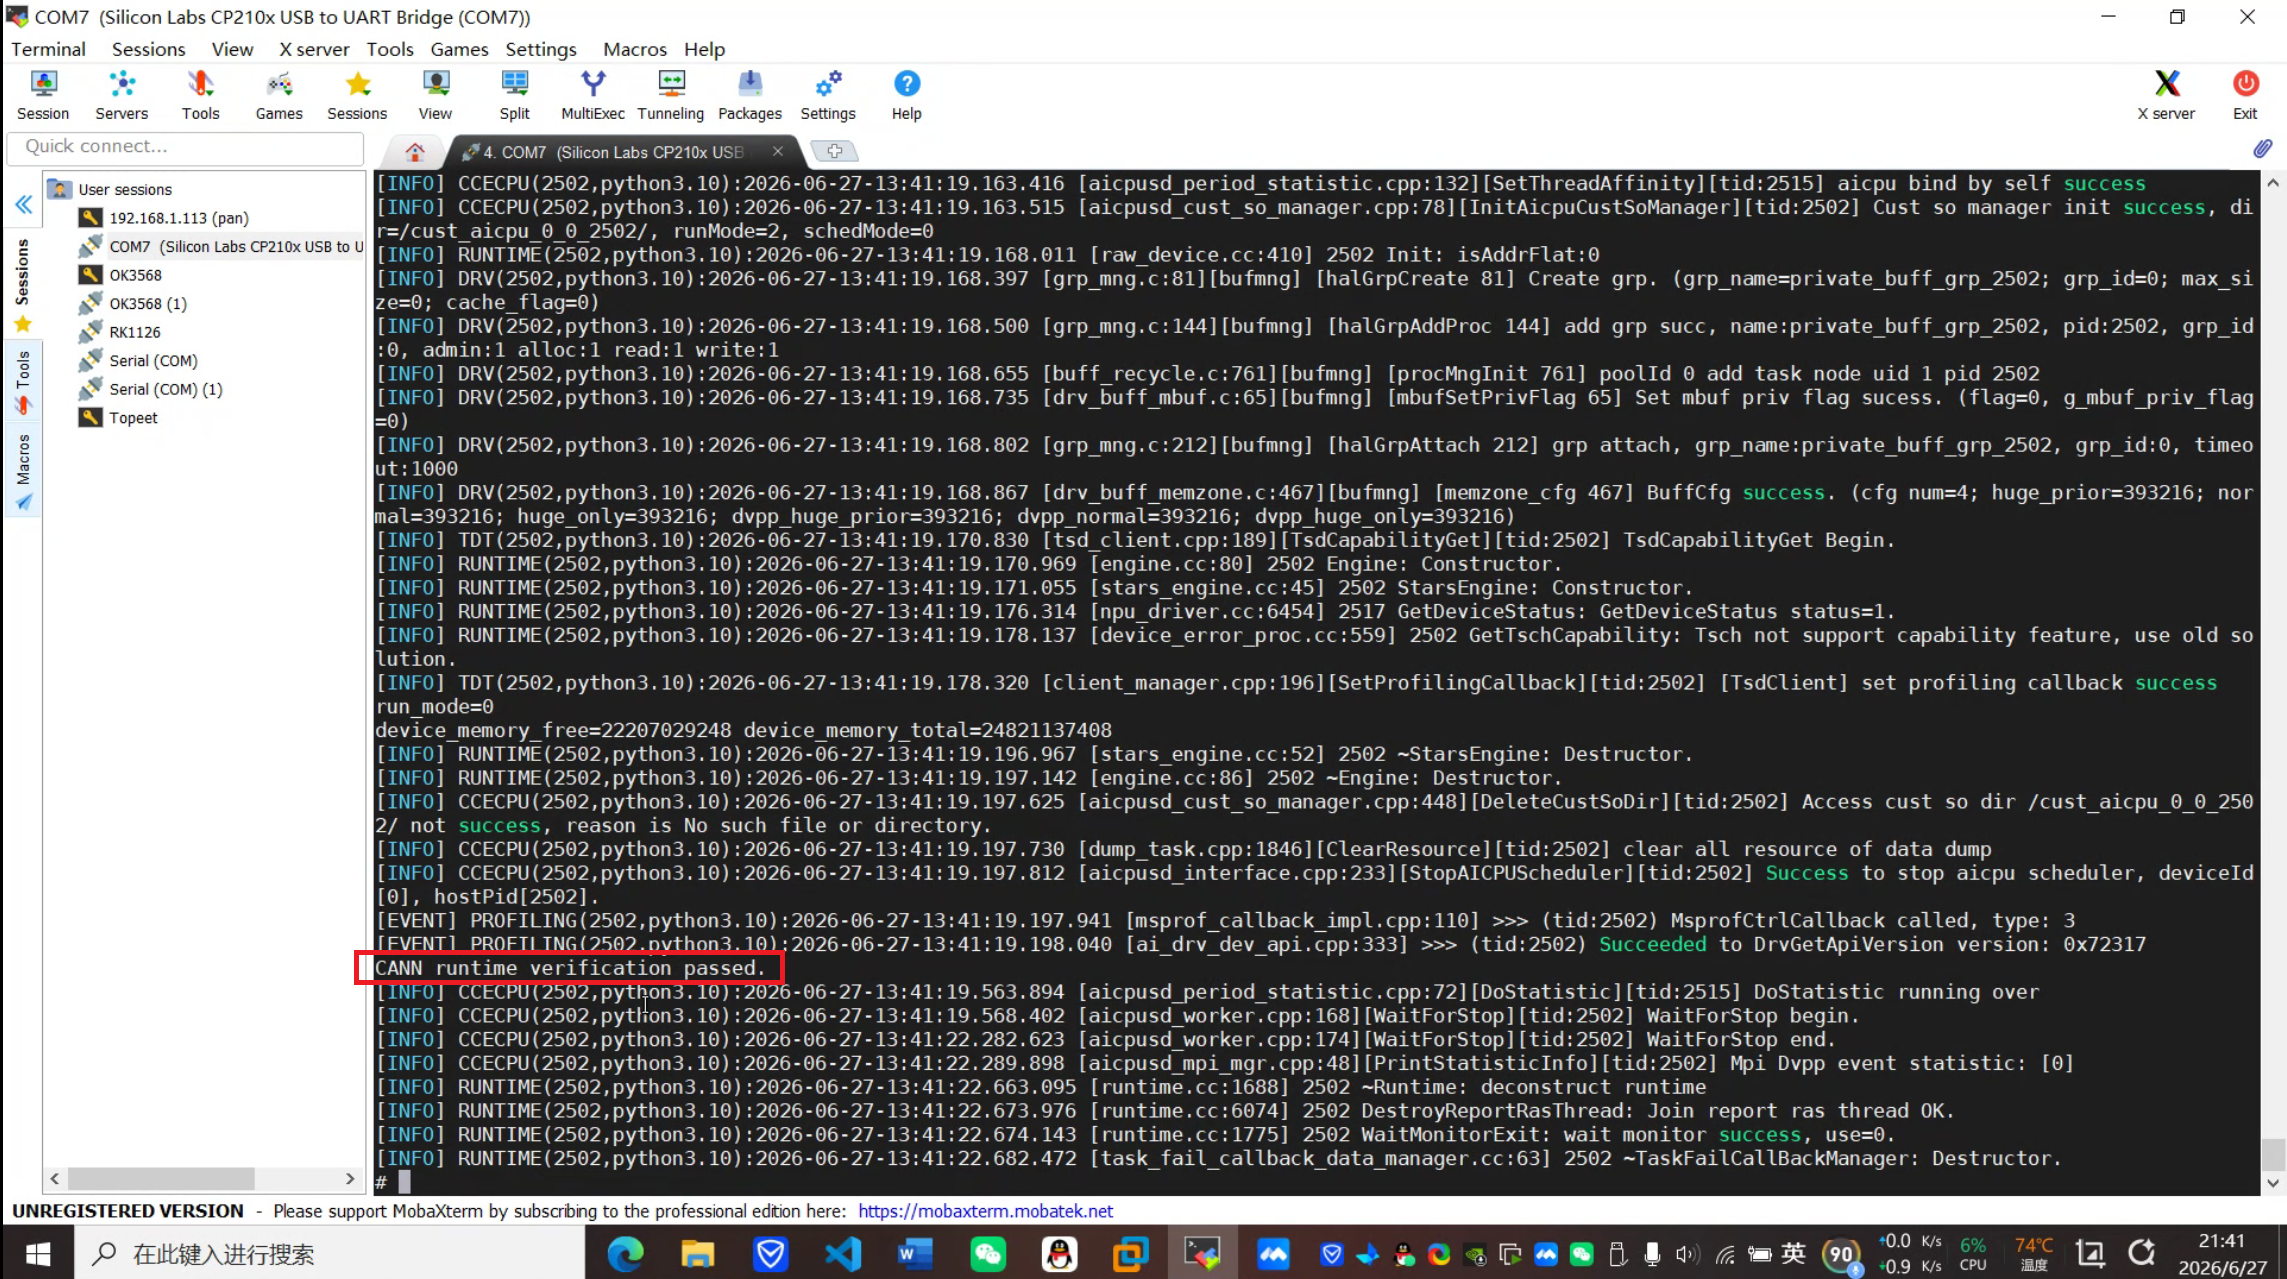
\includegraphics[width=0.8\textwidth]{verification.png}
  \caption{脚本验证结果}
  \label{fig:verification}
\end{figure}